\documentclass[11pt, a4paper,slovak]{article}
\usepackage[utf8]{inputenc}
\usepackage[slovak]{babel}
\usepackage[a4paper, text={17cm, 24cm}, left=2cm, top=3cm]{geometry}
\usepackage{graphicx} 
\usepackage{listings}
\usepackage{subfigure}
\usepackage{xcolor}
\usepackage{float}
\usepackage{amsmath}
\usepackage{xurl}

\lstset{
    basicstyle=\ttfamily\small,
    breaklines=true,
    frame=single,
    language=C,
    commentstyle=\color{gray},
    keywordstyle=\color{blue},
    stringstyle=\color{red}
}

\begin{document}
\begin{titlepage}
\begin{center}


\begin{figure}[h]
    \centering
    
\includegraphics[width=0.7\textwidth]{fig/logo_cz.png}
    \label{fig:enter-label}
\end{figure}
\vspace{\stretch{0.418}}
\Huge IMP – Mikroprocesorové a vestavěné systémy\\  
\huge Měření vzdálenosti/rychlosti pomocí ultrazvuku\\ [1em]
\large{
Hugo Bohácsek 
}
\vspace{\stretch{0.618}}
\end{center}
{\Large {2025/2026 \hfill xbohach00}}
\end{titlepage}
\newpage 

\tableofcontents

\newpage 

\section{Úvod}

Meranie vzdialenosti pomocou ultrazvuku patrí medzi bežné aplikácie vstavaných systémov. Ultrazvukové senzory nachádzajú uplatnenie na dŕahe, v robotike, automatizácii, parkovacích asistentoch, či priemyselnej meracej technike. Ich výhodou je bezkontaktný princíp merania, dostatočná presnosť pre väčšinu aplikácií a relatívne nízka cena.

\subsection{Motivácia}

Cieľom tohto projektu bolo vytvorenie kompletnej vstavanej aplikácie pre mikrokontrolér NXP Kinetis K60 (MK60DN512ZVMD10) - fitkit v3, ktorá umožňuje meranie vzdialenosti pomocou ultrazvukového senzora a poskytuje používateľovi prehľadné zobrazenie nameraných hodnôt spolu s možnosťou konfigurácie. Projekt využíva hardvérové časovače, prerušenia a multiplexovanie displeja bez použitia blokujúcich oneskorení.


\newpage
\section{Rozbor a návrh riešenia}

\subsection{Použitá platforma a komponenty}

Projekt bol realizovaný na výukovej platforme FITkit3 (varianta Minerva1) osadenej mikrokontrolérom NXP Kinetis K60 (MK60DN512ZVMD10) s jadrom ARM Cortex-M4.

\subsubsection{Ultrazvukový senzor}

Pre meranie vzdialenosti bol použitý ultrazvukový senzor HY-SRF05, ktorý pracuje na princípe merania doby prechodu ultrazvukového signálu. Senzor disponuje dvoma pinmi:
\begin{itemize}
    \item \texttt{TRIG} -- vstupný pin pre spustenie merania (min. 10~µs pulz)
    \item \texttt{ECHO} -- výstupný pin, ktorého dĺžka pulzu zodpovedá nameranej vzdialenosti
\end{itemize}

Merací rozsah senzora je 2--400~cm s uhlom záberu približne 15°. Vzdialenosť sa vypočíta zo vzťahu:
\[ \text{vzdialenosť}[\text{cm}] = \frac{\text{dĺžka ECHO pulzu}[\mu\text{s}]}{58} \]

\subsubsection{Sedemsegmentový displej}

Pre zobrazenie nameranej hodnoty bol použitý štvormiestny sedemsegmentový displej HS410561K-32. Displej je riadený technikou multiplexovania -- v každom okamihu svieti len jedna číslica, ale vďaka rýchlemu prepínaniu je pre ľudské oko viditeľný celý výpis. Každá číslica je aktivovaná samostatným GPIO pinom a segmenty sú zdieľané.

\subsubsection{Ďalšie komponenty}

\begin{itemize}
    \item \textbf{Tlačidlá:} Pre ovládanie aplikácie sú použité vstavané tlačidlá SW2, SW3, SW5 a SW4
    \item \textbf{Piezo bzučiak:} Zapojený na pin PTA4, slúži na akustickú signalizáciu
\end{itemize}

\subsection{Princíp merania vzdialenosti}

Meranie vzdialenosti prebieha v nasledujúcich krokoch:

\begin{enumerate}
    \item \textbf{Spustenie merania:} Periodický časovač PIT2 každých 60~ms vyvolá prerušenie a spustí nové meranie
    \item \textbf{Generovanie TRIG pulzu:} Pin TRIG je nastavený do logickej 1, časovač PIT0 je spustený s hodnotou zodpovedajúcou 10~µs
    \item \textbf{Ukončenie TRIG pulzu:} Po uplynutí 10~µs prerušenie od PIT0 ukončí TRIG pulz (nastaví pin do logickej 0)
    \item \textbf{Detekcia ECHO signálu:} Prerušenie na porte A reaguje na nábežnú hranu ECHO signálu -- spustí časovač PIT1 pre meranie dĺžky pulzu a zároveň časovač pre timeout
    \item \textbf{Ukončenie merania:} Zostupná hrana ECHO signálu spustí prerušenie, ktoré uloží nameraný čas
    \item \textbf{Výpočet vzdialenosti:} Nameraný čas je prepočítaný na vzdialenosť v~centimetroch
\end{enumerate}

V prípade, že ECHO signál nie je prijatý do 30~ms, meranie je automaticky ukončené a vzdialenosť zostáva nezmenená.

\newpage
\section{Vlastné riešenie}
\subsection{Schéma zapojenia}
\begin{figure}[H]
    \centering
    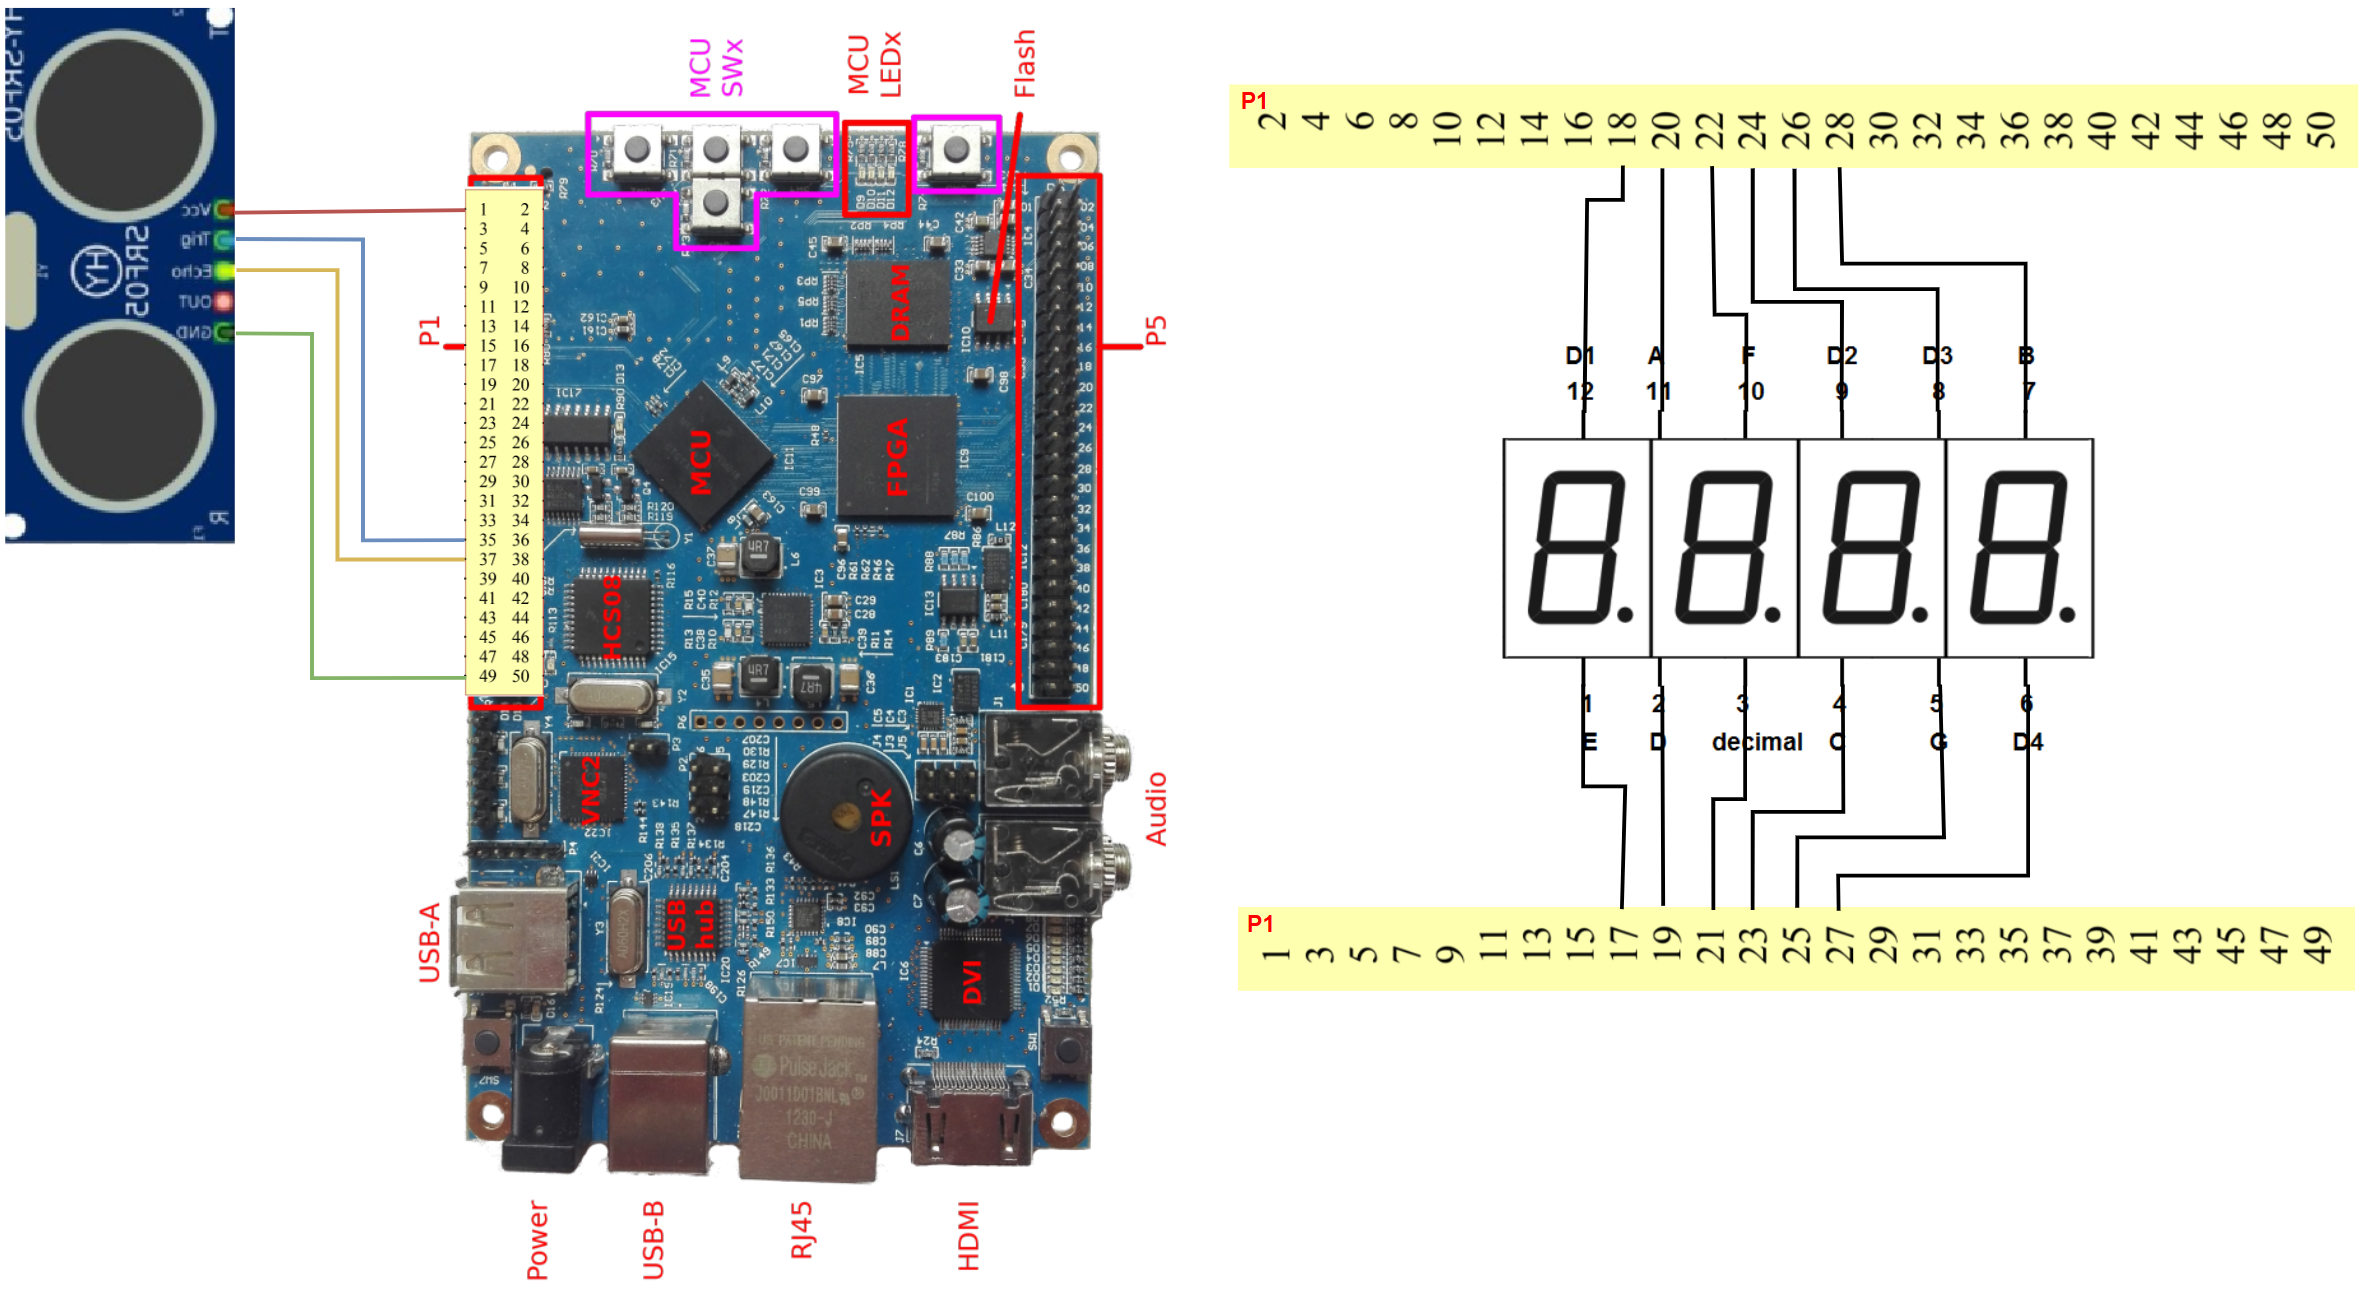
\includegraphics[width=\textwidth]{fig/diagram.png}
    \caption{Schéma zapojenia, pre väčšiu prehľadnosť oddelená}
\end{figure}

\subsection{Inicializácia mikrokontroléra}

Inicializácia systému prebieha vo funkcii \texttt{main()} a zahŕňa:
\begin{enumerate}
    \item Nastavenie hodinového signálu mikrokontroléra
    \item Konfiguráciu GPIO portov
    \item Inicializáciu a spustenie časovačov
\end{enumerate}

\subsubsection{Nastavenie hodinového signálu}

Mikrokontrolér je nakonfigurovaný pre prácu s taktom 50~MHz na zbernici. Toto nastavenie zabezpečuje dostatočný výkon pri zachovaní nízkej spotreby energie:

\begin{lstlisting}
void MCUInit(void) {
    MCG->C4 |= (MCG_C4_DMX32_MASK | MCG_C4_DRST_DRS(0x01));
    SIM->CLKDIV1 |= SIM_CLKDIV1_OUTDIV1(0x00);
    WDOG->STCTRLH &= ~WDOG_STCTRLH_WDOGEN_MASK;
}
\end{lstlisting}

\subsubsection{Konfigurácia GPIO}

Všetky použité piny sú nakonfigurované s príslušným multiplexorom (MUX) a v prípade výstupných pinov aj so zvýšenou výstupnou silou (DSE) pre spoľahlivé riadenie pripojených komponentov. U kritických signálov (napríklad ovládanie displeja) je navyše povolené obmedzenie rýchlosti prebehu (SRE) pre zníženie elektromagnetického rušenia.

\subsection{Meranie vzdialenosti}

Jadro meracieho systému tvoria dvojica funkcií \texttt{send\_trig()} a \texttt{receive\_echo()}.

\subsubsection{Generovanie TRIG pulzu}

Funkcia \texttt{send\_trig()} inicializuje nové meranie:

\begin{lstlisting}
static inline void send_trig(void) {
    echo_valid = 0;
    GPIO_SET(GPIOA, PIN_TRIG);
    PIT_STOP(0);
    PIT_CLEAR_FLAG(0);
    PIT_START(0);
}
\end{lstlisting}
Časovač PIT0 je vopred nastavený na hodnotu zodpovedajúcu 10~µs. Po jeho uplynutí dôjde k prerušeniu:

\begin{lstlisting}
void PIT0_IRQHandler(void) {
    PIT_CLEAR_FLAG(0);
    GPIO_CLEAR(GPIOA, PIN_TRIG);
    PIT_STOP(0);
}
\end{lstlisting}

\subsubsection{Príjem a spracovanie ECHO signálu}

Detekcia ECHO signálu je realizovaná prerušením na porte A:

\begin{lstlisting}
void PORTA_IRQHandler(void) {
    if (!(PORTA->ISFR & PIN_ECHO)) return;
    PORT_CLEAR_FLAG(PORTA, PIN_ECHO);

    if (GPIO_READ(GPIOA, PIN_ECHO)) {
        // Nabezna hrana - start merania
        PIT_STOP(1);
        PIT_CLEAR_FLAG(1);
        PIT_START(1);
    } else {
        // Zostupna hrana - koniec merania
        if (PIT_IS_RUNNING(1)) {
            echo_ticks = PIT_GET_ELAPSED(1);
            echo_valid = 1;
            PIT_STOP(1);
        }
    }
}
\end{lstlisting}
Výpočet vzdialenosti prebieha v hlavnej slučke:

\begin{lstlisting}
static inline void receive_echo(void) {
    if (!echo_valid) return;

    uint32_t ticks_local = echo_ticks;
    echo_valid = 0;

    uint32_t pulse_us = 
        (uint32_t)(((uint64_t)ticks_local * 1000000ULL) / BUS_CLK_HZ);
    distance = pulse_us / 58;
}
\end{lstlisting}
Pre prevenciu pretečenia je použitý 64bitový medzivýpočet s následným prevodom na 32 bitov.

\subsection{Zobrazenie na sedemsegmentovom displeji}

Zobrazenie je realizované multiplexovaním v prerušení časovača PIT3, ktoré je volané každé 4~ms (250~Hz).

\subsubsection{Prevod číslice na segmenty}

Pre každú číslicu 0--9 je definovaná štruktúra obsahujúca masku pre segmenty na porte A a porte D:

\begin{lstlisting}
typedef struct {
    uint32_t a;  // Segmenty na PORTA
    uint32_t d;  // Segmenty na PORTD
} seg_pattern_t;

static const seg_pattern_t seg_patterns[10] = {
    SEG_PATTERN_0, SEG_PATTERN_1, ..., SEG_PATTERN_9
};
\end{lstlisting}
Napríklad pre číslicu „8" je potrebné rozsvietiť všetky segmenty okrem desatinnej bodky:

\begin{lstlisting}
#define SEG_PATTERN_8 { \
    .a = SEG_B | SEG_C | SEG_G, \
    .d = SEG_A | SEG_D | SEG_E | SEG_F \
}
\end{lstlisting}

\subsubsection{Multiplexovanie}

V prerušení PIT3 je postupne aktivovaná každá číslica:

\begin{lstlisting}
void PIT3_IRQHandler(void) {
    PIT_CLEAR_FLAG(3);
    ticks++;

    DIGITS_ALL_OFF();
    SEGMENTS_ALL_OFF();

    uint8_t pos = disp_pos;
    disp_pos = (disp_pos + 1) & 3;  // Rotacia 0-3

    display_digit(disp_digits[pos], 0);
    digit_on(pos + 1);
    
    // ... obsluha bzuciaka ...
}
\end{lstlisting}
Najprv sú vypnuté všetky číslice a segmenty, potom je nastavená maska segmentov pre aktuálnu číslicu a nakoniec je aktivovaná príslušná číslica. Tento postup zabraňuje ghostingu (presvitu) medzi číslicami.

\subsection{Používateľské rozhranie}

\subsubsection{Obsluha tlačidiel}

Tlačidlá sú obslúžené v prerušení portu E s implementovaným softvérovým debouncingom:

\begin{lstlisting}
void PORTE_IRQHandler(void) {
    int flags = PORTE->ISFR & BTN_MASK;
    int now = ticks;

    PORT_CLEAR_FLAG(PORTE, flags);
    if (flags == 0) return;

    if ((now - last_btn) < SW_DEBOUNCE) return;
    last_btn = now;

    if (flags & BTN_BUZZ) {
        buzzer_enabled ^= 1;
    }

    if (flags & BTN_MODE) {
        ui_state = (ui_state == S_NORMAL) 
                  ? S_CFG : S_NORMAL;
    }

    if (ui_state == S_CFG) {
        if (flags & BTN_UP) {
            threshold = (threshold + STEP_THRESHOLD <= MAX_THRESHOLD)
                        ? threshold + STEP_THRESHOLD : MAX_THRESHOLD;
        }
        if (flags & BTN_DOWN) {
            threshold = (threshold >= MIN_THRESHOLD + STEP_THRESHOLD)
                        ? threshold - STEP_THRESHOLD : MIN_THRESHOLD;
        }
    }
}
\end{lstlisting}
Debouncing zabezpečuje, že medzi dvoma stlačeniami musí uplynúť minimálne 150 cyklov systémového času (približne 600~ms pri frekvencii 4~ms).

\subsubsection{Funkcia tlačidiel}

\begin{itemize}
    \item \textbf{SW4 - ľavé (BTN\_BUZZ):} Zapnutie/vypnutie bzučiaka
    \item \textbf{SW2 - pravé (BTN\_MODE):} Prepnutie medzi režimom merania a nastavenia
    \item \textbf{SW5 - nahor (BTN\_UP):} Zvýšenie prahovej hodnoty (v režime nastavenia)
    \item \textbf{SW3 - nadol (BTN\_DOWN):} Zníženie prahovej hodnoty (v režime nastavenia)
\end{itemize}

\newpage
\section{Záverečné zhodnotenie}

\subsection{Splnenie požiadaviek zadania}

Projekt úspešne spĺňa povinné požiadavky zadania:
\begin{itemize}
    \item Bola vytvorená funkčná aplikácia pre meranie vzdialenosti pomocou ultrazvukového senzora HY-SRF05
    \item Nameraná hodnota je zobrazovaná na štvormiestnom sedmosegmentovom displeji
    \item Aplikácia umožňuje používateľovi konfiguráciu prahovej hodnoty pomocou tlačidiel
    \item Akustická signalizácia pomocou piezo bzučiaka reaguje na vzdialenosť od nastaveného prahu
    \item Systém rozlišuje, či je meranie v rámci alebo mimo nastaveného rozsahu
\end{itemize}

\subsection{Technické aspekty implementácie}

Aplikácia bola navrhnutá s dôrazom na efektívne využitie hardvérových prostriedkov mikrokontroléra. Všetky časovo kritické operácie sú riešené pomocou hardvérových časovačov a prerušení, čo zabezpečuje presné časovanie bez blokovania procesora. Multiplexovanie displeja prebieha dostatočne rýchlo (250~Hz na číslicu), aby nebolo ľudským okom vnímané blikanie.

Implementácia debouncingu tlačidiel softvérovo v prerušení sa ukázala ako dostatočne spoľahlivá pre bežné použitie. Systém je odolný voči rušeniu vďaka použitiu timeout mechanizmu pri meraní ECHO pulzu.

\subsection{Problémy pri riešení}

Počas implementácie bolo nutné vyriešiť niekoľko technických problémov:

\textbf{Pretečenie pri výpočte vzdialenosti:} Počiatočná implementácia používala 32bitovú aritmetiku, čo viedlo k pretečeniu pri násobení. Problém bol vyriešený použitím 64bitového medzivýpočtu s explicitným pretypovaním.

\textbf{Ghosting na displeji:} Pri nedostatočne rýchlom vypnutí predchádzajúcej číslice pred aktiváciou ďalšej dochádzalo k presvitu segmentov. Riešením bolo explicitné vypnutie všetkých číslic a segmentov pred nastavením novej hodnoty.

\textbf{Časovanie TRIG pulzu:} Pre spoľahlivú funkciu senzora je nutné dodržať minimálnu dĺžku TRIG pulzu 10~µs. Použitie hardvérového časovača zabezpečuje presné časovanie nezávisle na zaťažení procesora.

\textbf{Slabo svietace segmenty D a F:} Toto sa mi žiaľ nepodarilo úplne odstrániť. Vybrané piny sú zdieľané s vyskoko rýchlostnými perifériami, sú teda vysokokapacitné a slabšie. Zároveň sa fitkit z neznámych dôvodov reštartuje pri zatlaćení na ne, čo tiež nepomohlo ladaniu.

\newpage
\section{Použité informačné zdroje}

\subsection{Technická dokumentácia}

\begin{enumerate}
    \item \textbf{K60 Sub-Family Reference Manual}, Rev. 2, Freescale Semiconductor, 2012. \\
    Komplexná referenčná príručka k mikrokontroléru MK60DN512ZVMD10 obsahujúca detailný popis všetkých periférií, registrov a ich použitia.
    
    \item \textbf{K60 Sub-Family Data Sheet}, Rev. 7, Freescale Semiconductor, 2013. \\
    Datasheet obsahujúci elektrické parametre, pinout a základné technické špecifikácie mikrokontroléra.
    
    \item \textbf{HY-SRF05 Ultrasonic Sensor Module Datasheet}. \\
    Technická dokumentácia k ultrazvukovému senzoru HY-SRF05
    
    \item \textbf{HS410561K-32 Common Anode 4-Digit 7-Segment Display Datasheet}. \\
    Špecifikácia sedmosegmentového displeja vrátane elektrických parametrov a pinoutu.
\end{enumerate}

\subsection{Vývojárske nástroje a SDK}

\begin{enumerate}
    \setcounter{enumi}{4}
    \item \textbf{MCUXpresso IDE User Guide}, NXP Semiconductors. \\
    Dokumentácia k vývojovému prostrediu použitému pre vývoj a ladenie aplikácie.
    
    \item \textbf{ARM Cortex-M4 Generic User Guide}, ARM Limited. \\
    Referenčná príručka k architektúre ARM Cortex-M4 obsahujúca popis inštrukčnej sady a systémových periférií.
    
    \item \textbf{FITkit3 quickstart}, FIT VUT v Brně. \\
    Schémy zapojenia a technická dokumentácia výukovej platformy FITkit3 dostupná z: \\
    \url{https://git.fit.vut.cz/strnadel/edu/src/branch/main/howto-hints/embedded/FITkit3_dev_quickstart_cz.md}
\end{enumerate}

\subsection{Odborné zdroje a fóra}

\begin{enumerate}
    \setcounter{enumi}{7}
    \item \textbf{NXP Community Forums}, NXP Semiconductors. \\
    Diskusné fóra zamerané na mikrokontroléry Kinetis, príklady použitia periférií a riešenia problémov.
    
    \item \textbf{Embedded Systems Programming Articles}, \url{Embedded.com}. \\
    Odborné články o programovaní vstavaných systémov, best practices a optimalizačných technikách.
    
    \item \textbf{Application Note AN4445: Using PIT Module in Kinetis}, Freescale Semiconductor. \\
    Aplikačná poznámka popisujúca použitie časovačov PIT vrátane príkladov kódu a odporúčaných postupov.
\end{enumerate}

\subsection{Prevzaté časti riešenia}

V projekte boli použité nasledujúce časti kódu prevzaté z externých zdrojov:

\begin{itemize}
    \item \textbf{Inicializácia MCU a hodinového signálu:} Kód bol inšpirovaný príkladmi z oficiálneho SDK pre Kinetis K60 od NXP Semiconductors (Freedom board examples).
    
    \item \textbf{Makrá pre prácu s GPIO a PIT:} Definície makier pre zjednodušenie prístupu k registrom boli vytvorené na základe odporúčaní z ARM Cortex-M Programming Guide a Application Note AN4445.
    
    \item \textbf{Výpočet vzdialenosti z ECHO pulzu:} Vzorec pre prevod dĺžky pulzu na vzdialenosť je štandardný pre ultrazvukové senzory a je uvedený v datasheete HY-SRF05.
\end{itemize}

\end{document}
